\chapter{Diskretes Äußeres Kalkül (DEC)}
\label{chapterDEC}

see \cite{Lee} \cite{FirstCourse}

\section{Diskrete Differentialformen}
  
  \begin{definition}
    Eine diskrete \( p \)-Form ist ein Homomorphismus vom Kettenkomplex \( C_{p}(K) \) nach \( \R \).
    Die Menge aller dieser Homomorphismen bezeichnen wir je nach Kontext mit \( C^{p}(K) \) (Menge der \( p \)-Koketten)
    oder \( \Omega^{p}_{d}(K) \) (Menge der diskrete \( p- \)(Differential-)Formen). 
    Das heißt
    \begin{align}
      \hom(C_{p}(K),\R) =: C^{p}(K) =: \Omega^{p}_{d}(K) \formpunkt
    \end{align}
    Desweiteren erfolgt die Addition punktweise, das heißt
    \begin{align}
      \left( \alpha + \beta \right)(c) &:= \alpha(c) + \beta(c)
    \end{align}
    für \( \alpha,\beta \in C^{p}(K) \) und \( c \in C_{p}(K) \).
  \end{definition}
  
  \begin{folgerung}
    \label{folgUnikKoketten}
    Da \( \R \) mit der Addition eine abelsche Gruppe ist, können wir uns wieder die Universalitätseigenschaft \eqref{diagFreieAbelscheGruppe} des Kettenkomplexes zunutze machen.
    Für eine \( p \)-Kette \( c = \sum_{\sigma\in K^{(p)}} a_{\sigma} \sigma \in C_{p}(K)\) und eine  \( p \)-Kokette \( \alpha\in C^{p}(K) \) gilt
    \begin{align}
      \alpha(c) &= \alpha\left(\sum_{\sigma\in K^{(p)}} a_{\sigma} \sigma\right) = \sum_{\sigma\in K^{(p)}} a_{\sigma} \alpha(\sigma) \formkomma
    \end{align}
    damit reicht es auch hier aus die \( p \)-Koketten nur auf den \( p \)-Simplizes zu definieren.
  \end{folgerung}

  Hätten wir die Menge der \( p \)-Ketten als \( \R \)-Vektoraum eingeführt, so hätte uns die Frage nach einem inneren Produkt zwischen den Ketten und den Koketten zur dualen Paarung
  geführt und damit auch, dass \( C^{p}(K) = \left( C_{p}(K) \right)^{*}\) der Dualraum von \( C_{p}(K) \) ist.
  Nun hält uns aber auch nichts davon ab, dies auch für die hier eingeführten Ketten analog zu machen.

  \begin{definition}
    \begin{align}
      \begin{aligned}
        \left\langle \bullet,\bullet \right\rangle : C^{p}(K) \times C_{p}(K)  &\rightarrow \R \\
                                                     \left( \alpha, c  \right) &\mapsto \left\langle \alpha, c \right\rangle := \alpha(c)
      \end{aligned}
    \end{align}
    heißt natürliche Paarung zwischen den \( p \)-Koketten (-Formen) und den \( p \)-Ketten.
  \end{definition}

  Die Verbindung zwschen diskreter Form und Differentialform ist die de-Rham-Abbildung.
  Dazu nehmen wir zunächst an, dass wir einen abstrakten Simplizialkomplex \( L \) vorliegen haben, das heißt, dass alle Simplizes auf der zugehörigen Mannigfaltigkeit \( M \) liegen.
  Das bringt erst einmal den Vorteil, dass Integration auf den Simplizes das gleiche Ergebinis auch auf der Mannigfaltigkeit liefert.

  \begin{definition}
    Die de-Rham-Abbildung bildet \( p \)-Differentialformen auf diskrete \( p \)-Formen (Koketten) ab. 
    Genauer
    \begin{align}
      \begin{aligned}
        \psi^{p}: \Omega^{p}(M) &\rightarrow C^{p}(L) = \Omega_{d}^{p}(L)\\
                       \alpha   &\mapsto \left( \sigma^{p} \mapsto \int_{\sigma^{p}} \alpha =: \psi^{p}(\alpha)(\sigma^{p}) =  \left\langle \psi^{p}(\alpha), \sigma^{p} \right\rangle\right)
                       \formkomma
      \end{aligned}
    \end{align}
    das heißt die diskrete \( p \)-Form \( \psi^{p}(\alpha) \in \Omega_{d}^{p}(L)  \) ist auf den \( p \)-Simplizes definiert, was wegen Folgerung \ref{folgUnikKoketten} vollkommen ausreicht.
  \end{definition}

  Da das Integral ein lineares Funktional ist, ist auch \( \psi \) linear.
  \todo{whitney abbildung noch ansprechen? Das heißt Interpolation im allgemeinen oder nur speziell?}

  \begin{bemerkung}
    Nun haben wir bei der Definition der de-Rham-Abbildung vorrausgesetzt, dass ein abstrakter Simplizialkomplex vorliegt.
    Das entspricht aber nur für flache Mannigfaltigkeiten unseren Anfoderungen.
    Im Allgemeinen ist die gegebene Triangulation nur eine lineare Approximation der Mannigfaltigkeit und damit auch des zugehörigen abstrakten Simplizialkomplexes.
    Das bedeutet auch, dass für \( p \ge 1 \) die Differentialformen von \( M \) in einem anderen Raum "`leben"' als die Differentialformen des Polytopes \( |K| \).
    Für die numerische Analysis ist das eine schwierige Situation, da vor der eigentlichen Diskretisierung (Diskretisierungsfehler) noch eine Approximation (geometrischer Fehler) auf einen stückweise
    flachen Raum gemacht wird.

    Für \( 0 \)-Formen (identisch zu Skalarfeldern) ergibt sich dieser geometrische Fehler nicht, da nach Vorraussetzung die Ecken des Simplizialkomplexes auf der Mannigfaltigkeit liegen.
    Hier ist die Diskretisierung genauso wie wir das aus anderen Verfahren, wie die Finite-Differenzen-Methode, gewöhnt sind, da das "`Punktintegral"' nichts weiter als die Auswertung an
    eben diesem Punkt ist.
    Das heißt, liegt ein Skalarfeld \( u:M\rightarrow\R \) vor, so ist das diskrete Skalarfeld \( u_{d}:K^{(0)} \rightarrow \R \) an den Ecken definiert.
    \begin{align}
      u(v_{i}) &=  \psi(u)(v_{i}) = \left\langle \psi(u), v_{i} \right\rangle= u_{d}(v_{i}) =: u_{i} 
    \end{align}
    für alle \( v_{i} \in K^{(0)} \).
    Die Interpolation zurück zur Mannigfaltigkeit kann dann mittels linearer Ansatzfuktionen erfolgen, die sich auf den abstrakten Volumenenelementen \( \pi(\sigma^{n}) \) definieren.
    \( \pi \) ist hier wieder die Projektion.
    \begin{figure}
      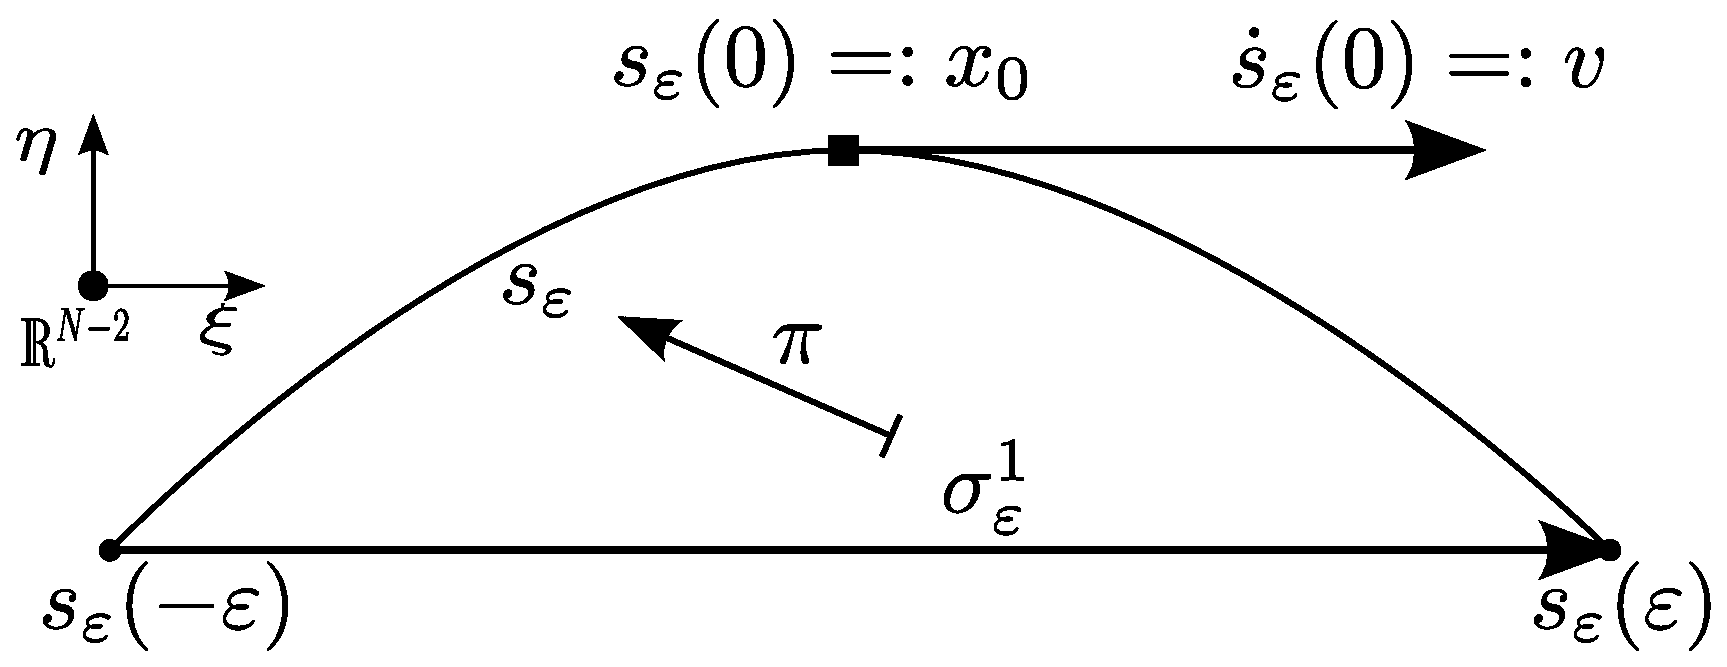
\includegraphics[width=\textwidth]{bilder/EpsilonKette.eps}
      \caption[Fehler bei der Auswertung diskreter 1-Form]{sadsad}
      \label{figDiskrete1Form}
    \end{figure}
  \end{bemerkung}




  
  

\section{Äußere Ableitung}
  

  

  

\section{Hodge-Operator}

\section{Laplace-Operator}

  \subsection{Beispiel: Laplace-Gleichung}

  \subsection{Beispiel: Krümmung Teil 1: Gauß-Bonnet-Operator}
  \subsection{Beispiel: Krümmung Teil 2: Weingarten-Abbildung}
  \subsection{Beispiel: Krümmung Teil 3: Krümmungsvektor}


\section{Lie-Ableitung und Jacobian}

  \subsection{Beispiel: Wirbelgleichung}


